
\chapter{3D wings in compressible flows}
\section{The Prandtl-Glauert-Goethert transformation}
\subsection{Subsonic flows}
	The previous potential equation can be extended into 3D into the same conditions like: 
	
	\begin{equation}
	\beta ^2 \hat{\phi} _{xx} + \hat{\phi} _{yy} + \hat{\phi} _{zz} = 0.
	\end{equation}
	
	Then we apply the transformation of $(x, y, z)$ to $(X, y, z)$ with $X = \frac{x}{\beta}$ so that the previous equation becomes: 
	
	\begin{equation}
	\hat{\phi} _{XX} + \hat{\phi} _{yy} + \hat{\phi} _{zz} = 0.
	\end{equation}
	
	\wrapfig{7}{l}{6}{0.07}{ch7/1}{ch7/1}
	The flow in $(x,y,z)$ is compressible with $M<1$, when in $(X,y,z)$ it is incompressible. The solution or $\phi$ in similar points (points $x,y,z$ and $x/\beta,y,z$) is the same. This kind of transformation is represented on the figure. We remark that the leading edges sweep and the aspect ratios are related as: 
	
	\begin{equation}
	\frac{\tan \sigma _0}{\sigma} = \frac{n}{m} = \frac{1}{\beta} \qquad \frac{AR_0}{AR} = \frac{b^S_0}{b^2S} = \frac{c}{c_0} = \beta. 
	\end{equation}
	
	The slope of the wing in the z-direction is the same in the two axis: 
	\begin{equation}
	\tan \theta \approx \theta = \frac{\hat{w}}{\hat{u}+V_\infty} \approx \frac{\hat{w}}{V_\infty}. 
	\end{equation}
	
	The pressure coefficient for small perturbations is known: 
	
	\begin{equation}
	C_p = -\frac{2\hat{\phi}_{x}}{V_\infty} = -\frac{1}{\beta}\frac{2\hat{\phi}_{X}}{V_\infty} = \frac{C_{p0}}{\beta}.
	\end{equation}
	
	We obtain the same equation as in 2D, whereas now the profiles are not identical! For the lift on a section (y = cst), we can compute the integral:
	
	\begin{equation}
	L' = \frac{1}{2} \rho _\infty V_\infty ^2\int _{LE} ^{TE} (c_{pl} - c_{pu})\, dx
= \frac{1}{2} \rho _\infty V_\infty ^2\int _{LE} ^{TE} \frac{c_{pl,inc} - c_{pu,inc}}{\beta} \beta\, dX = L_0'
	\end{equation}
	
	They are the same, whereas the lift coefficients respect $c_l' = \frac{c_{l0}'}{\beta}$. This is also valid for the lift curve slope. 
	
\subsection{Supersonic flows}
	In this case the potential equation becomes:
	
	\begin{equation}
	\lambda ^2 \hat{\phi} _{xx} + \hat{\phi} _{yy} + \hat{\phi} _{zz} = 0.
	\end{equation}
	
	If we apply the analogous transformation we have:
	
	\begin{equation}
	X = \frac{x}{\lambda} \qquad \Rightarrow  \hat{\phi} _{XX} + \hat{\phi} _{yy} + \hat{\phi} _{zz} = 0.
	\end{equation}
	
	This equation does not correspond anymore to the equation of an incompressible flow since $\lambda = \sqrt{M_\infty ^2 - 1}$ and to have $\lambda = 1$ we need $M_\infty = \sqrt{2}$, thus the new flow is a $M_\infty = \sqrt{2}$. The previously found relations with $\beta$ are valid for $\lambda$. 
	
\section{Swept wings}
	\minifig{ch7/2}{ch7/3}{0.15}{0.15}{0.3}{0.3}
	This is a technique used in order to increase the critical mach number. Indeed, the flow seen by the 2D wing is the one perpendicular to the wing:
	
	\begin{equation}
	V_{\infty n} = V_{\infty}\cos \sigma \qquad \Rightarrow M_{kr}^\sigma= \frac{M_{kr}^{\sigma = 0}}{\cos^m \sigma}
	\end{equation}
	
	where we can see that the $M_\infty$ will be higher and where m varying parameter in function of the $C_L$, it decreases with lift (\autoref{ch7/3}). if the sweep angle is large enough, the flow seen by the LE can become subsonic and allow rounded shapes which is advantageous for subsonic speeds. The drag divergence mach number also increases:
	
	\begin{equation}
	M_{div} = M_{kr} [1.02 + 0.08 (1-\cos \sigma)].
	\end{equation}
	
\subsection{Lift of swept wings}
	Remind the definition of $C_p$: 
	
	\begin{equation}
	C_{pn} = \frac{p-p_\infty}{\frac{1}{2} \rho _\infty V_{\infty n} ^2} \qquad L_n = \frac{1}{2}\rho _\infty V_{\infty n} ^2 \int _{LE} ^{TE} (C_{pln} - C_{pun}) \, dx 
	\end{equation}
	
	\wrapfig{11}{l}{4.5}{0.12}{ch7/4}{ch7/4}
	where we see that if $M_{\infty n} = M_\infty^*$ ($M_\infty^*$ in this case is the one we have without sweep), the pressure distribution and thus the lift remains constant. This means that for a same approaching speed $V_\infty^*$ without and with sweep we will decrease the lift (we have to fly at higher speed). The lift coefficient also decreases for $V_{\infty n} = V_\infty^*$:
	
	\begin{equation}
	c_{l}^* = \frac{L^*}{\frac{1}{2}\rho _\infty V_{\infty}^*} > c_{l} = \frac{L^*}{\frac{1}{2}\rho _\infty V_{\infty}}
	\end{equation}
	
	where $^*$ designate the same value in non swept wing. We see that the lift coefficient decreases. 
	
	\wrapfig{5}{l}{6}{0.15}{ch7/5}{ch7/5}
	Pay attention that this is the case when we are in subsonic flight. Indeed, the sweep increases the lift for supersonic as the shock stall is postponed ($M_{\infty n}$ seen smaller). In practice, to have significant influence of sweep $\sigma$ must be high (at least 30\degres - 40\degres). 
	
\subsection{Lift coefficient as a function of the angle of attack for swept wings}	
	\wrapfig{8}{r}{6}{0.15}{ch7/6}{ch7/6}
	As we have seen, the lift and the lift coefficient decreases when sweep wings. This implies that the slope of the lift curve is also smaller. Remark that we have the same AR in the figure, in practive the AR of swept wing is smaller than the one without (2 to 4 - sweep, 6 to 10 - subsonic), but the lift slope is even smaller. 
	
	\ \\ There are structural advantages as it allows to have thinner airfoils (better for high speed), and the $M_{kr}$ increases. To increase the structural strength we use \textbf{taper} (chord decreases from root to tip). This smaller AR induces more drag, demanding more take-off and landing distance. The reduced slope of lift requires high $\alpha$ when landing and take-off (Concorde drooped nose), but there is no pronounced stall limit.    
	
\subsection{Influence of the sweep angle on the drag}	
	\wrapfig{7}{l}{6}{0.1}{ch7/7}{ch7/7}
	One observes the increase of $M_{div}$, the decrease of the maximum drag coefficient (must have large angles to have significant effects). At sufficiently high Mach numbers, $M_n$ will reach the supersonic limit and produce the same effect as seen previously. In that case, the drag with no swept wing is smaller at this stage. 
	
	\ \\
	
\subsection{Some additional disadvantages of wings}
\subsubsection{Separation behavior}
	\wrapfig{9}{r}{6}{0.1}{ch7/8}{ch7/8}
 	First, remind that the pressure on the suction side decreases moving from the root to the tip, perpendicularly to the flow, inducing a flow. In practice, we try to have the separation at TE the nearest to the root not to disturb the ailerons (or else loose of control). The problem is that as we are already beyond the peak of underpressure at the root, to the tip we reach the underpressure, thus the boundary layer is pushed to the tip, resulting in a flow of low velocity and low energy. This will separate easily. 
 	
 	\minifig{ch7/9}{ch7/10}{0.12}{0.1}{0.35}{0.3}
 	
 	Solutions to limit this are: 
 	
 	\begin{itemize}
 	\item[•] \textbf{washout}: we make the geometry in order to reduce $\alpha$ when going to the tip and increase the speed.
 	
 	\item[•] \textbf{separation at root}: we force it to happen there for example by sharp LE
 	
 	\item[•] \textbf{use of slots and slats} (see further)
 	
 	\item[•] \textbf{stall fences}: it is a device placed on the wing in order to brake the flow going from root to tip (\autoref{ch7/9}).
 	\end{itemize}
 	
\subsubsection{Efficiency of flaps and ailerons}
	Flaps are devices made to increase the lift, used in take-off and landing. The flaps become less effective with sweep. For example, a slotted over 60\% span can increase the lift coefficient about 50\% for non swept and only 20\% for swept wings. This is why the part of the wing containing the flaps is not swept.  
	
	\begin{center}
	\begin{minipage}{0.33\textwidth}
	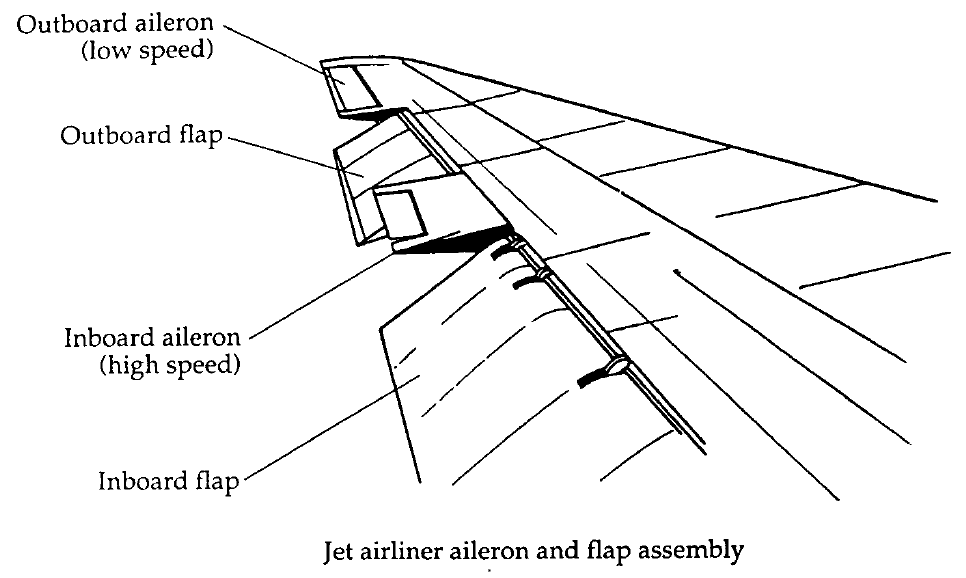
\includegraphics[scale=0.15]{ch7/11}
	\captionof{figure}{}
	\label{ch7/11}
	\end{minipage}
	\begin{minipage}{0.25\textwidth}
	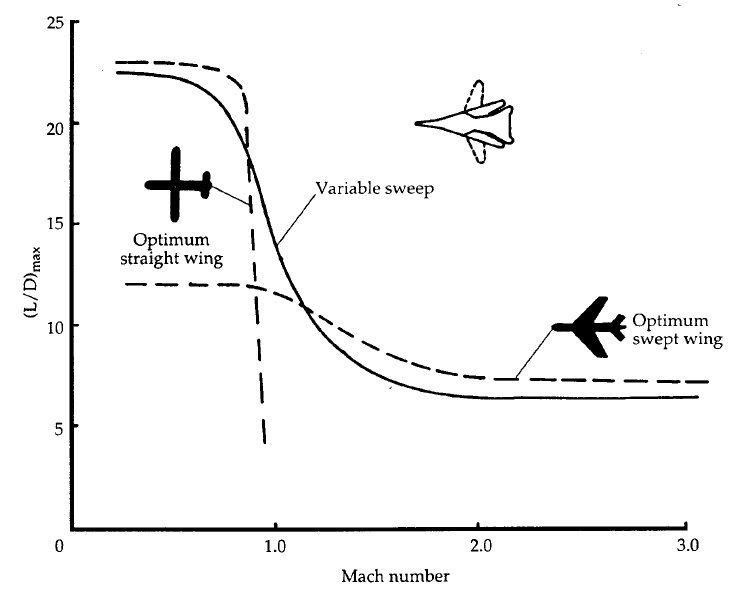
\includegraphics[scale=0.15]{ch7/12}
	\captionof{figure}{}
	\label{ch7/12}
	\end{minipage}
	\begin{minipage}{0.3\textwidth}
	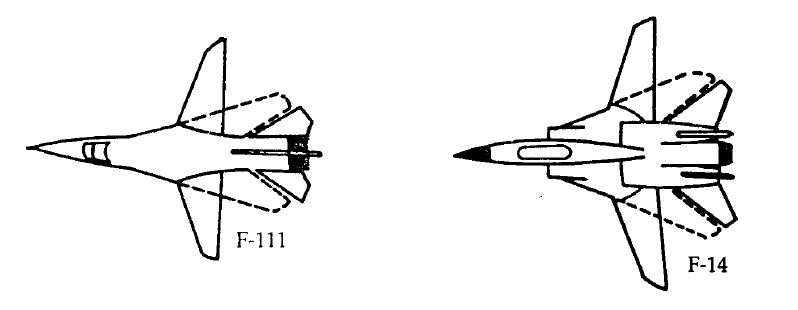
\includegraphics[scale=0.2]{ch7/13}
	\captionof{figure}{}
	\label{ch7/13}
	\end{minipage}
	\end{center}		
	
	This reduction of efficiency also occurs with the ailerons. We can conclude that it is better for a plane flying only at subsonic speeds to have no sweep, and better to have sweep for supersonic. We can have a \textbf{swing-wing} which is the variable sweep. 
	
	\wrapfig{6}{l}{3}{0.1}{ch7/14}{ch7/14}
	The \textbf{Forward Swept Wing (FSW)} has the same effect of the aft swept wing (ASW), but has advantages because the separation principle we have seen is reversed such that the separation occurs on the root $\rightarrow$ higher lift. At maximum lift, the FSW has an elliptic lift distribution along the wing, leading to less induced drag than the ASW which has a peak at the tip. This leads to a better efficiency of ailerons and flaps. 
	
	\ \\
	
	\wrapfig{5}{r}{4}{0.1}{ch7/15}{ch7/15} 
	But there is a structural instability. Indeed, the load is always accompanied with a bending of the wing. In straight case, there is no rotation of the profile. For the ASW the profile will move downward implying a decrease of the angle of attack (lift) and compensating the bending. In FSW the profile move upward, increasing $\alpha$ and the lift, causing more bending and so on $\rightarrow$ unstable. This can be avoided by sufficient structural strength. 
	
\subsubsection{Swept wing and supersonic flow}
	\minifig{ch7/16}{ch7/17}{0.1}{0.15}{0.35}{0.3}
	For high enough speeds, the normal mach number will be supersonic, we'll get \textbf{supersonic leading edge}. There will be appearance of the Mach cone, the flow at point A is only influenced by the blue area and it influences the green area. We can go to the tip, we see that it only influences a small part of the wing. The rest of the wing see 2D flow. To avoid the effect of the tip, we cut the region of influence, they are thus inefficient at subsonic and low supersonic speeds
	
\section{Area rule}
	\begin{center}
	\theor{
	\textbf{Theorem of Hayes}\\
	
	\textit{Within the limits of small perturbations, different planes with the same evolution of the area of their cross section will have the same wave drag at transonic Mach numbers (at zero lift).}
	}
	\end{center}
	
	\begin{center}
	\theor{
	\textbf{Whitcomb}\\
	
	\textit{In order to limit the wave drag for transonic flows, the variation of the area of the cross-section of a plane should be as smooth as possible, without abrupt changes.}
	}
	\end{center}
	
	\minifig{ch7/18}{ch7/19}{0.12}{0.12}{0.35}{0.3}
	
	\wrapfig{3}{l}{3}{0.15}{ch7/20}{ch7/20}
	This means that the cross section of the fuselage must be reduced near the tail in order to have that smooth variation. On this figure see the decrease and the late of the peak in drag around M=1 with area rule. 
	
	\newpage
\section{Delta wings}
	\wrapfig{9}{l}{5}{0.15}{ch7/21}{ch7/21}
	The idea of delta wings is to control the separation. By using a sharp LE one obtains a fixed separation line on LE. This is a considerably swept wing but has less problems with tip stall. This is due to the vorticies at the LE on the upper side that avoid the boundary layer to reach the tips. The separation area being limited, that produces an underpressure on the upper side and contributes to lift. 
	
	\ \\
	The slope of the lift curve is small, we can reach high $\alpha \approx 35\degres$. At still higher $\alpha$ the vorticies will lose their structure (\textbf{vortex burst}) and the underpressure will disappear, lift goes down. The large wings produce large lift and flaps are not needed. Tail plane are not necessary and the large chord at the root allows thick wings, keeping $t/c$ low, increasing structural strength, allowing fuel storage and engines integration (reduction of drag). To have good subsonic conditions, $b/l \approx 0.25$ or not smaller than 2.
	
\paragraph{Remark 1}
	This description only applies for subsonic LE. If it is supersonic there is no separation at the LE, there is a shock wave on the wing causing boundary layer separation.  
	
\paragraph{Remark 2}
	The lift creating process is different here. Joukowski theorem tells that it is based on vortex sheet, which is quasi horizontal for traditional wings. For delta wings the vortex sheet is rolled up. For wings with very low AR, $c_l$ in function of $\alpha$ is given by the \textbf{formula of Jones}:
	
	\begin{equation}
	c_l = \pi \alpha \frac{db}{dx}
	\end{equation}	 

	under the assumption that the wing lies perfectly in the Mach cone and where $\frac{db}{dx}=cst$ for delta wings. 
	
\paragraph{Remark 3}
	The vorticies cause the transition to turbulent flow. If one wants laminar flow boundary layer control is needed. 